\subsection{Example: Renting a car}
        In this section, an Alastria ID use case will be explained, which is the example that has been carried out in \acrshort{mvp}1\cite{mvp1-car}.\\
        
        In this example, a user (Subject) wants to rent a car, for this, the rental company (Service Provider) asks the user through a Presentation Request for three data: 1) the driving license, 2) his credit card and 3) prove that the user is over 25 years old. 
        \begin{figure}[h]
            \centering
            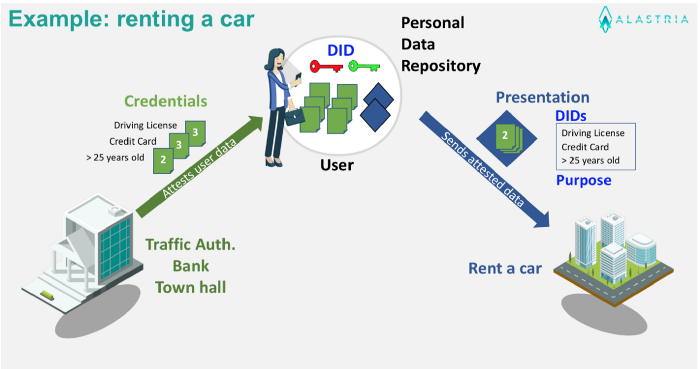
\includegraphics[width=0.8\textwidth]{ala-rent-car.png}
            \caption{Renting a car with Alastria ID}
            \label{fig:ex-car}
        \end{figure}
        The user must send this information to the rental company, and for this he uses Alastria ID and asks the Issuers at that time to certify that the user complies with these conditions. So the user asks the bank for his credit card, asks the traffic authority for his driving license and the town hall to verify he is over 25 years old. Each one of the Issuers (bank, traffic authority and town hall) sends the requested Credentials, and the user stores them in his wallet. The user, having all the needed data in the wallet, creates a Presentation in response to the Presentation Request above. The user sends the Presentation to the rental company. The rental company receives and validates it. Finally, it proceeds to provide the car to the user. All this process can be done directly online without the need for prior registration or verification of the original documents by the rental company. This example can be seen graphically in the figure \ref{fig:ex-car}.\\

        All these information flows between the different actors are registered in the blockchain with different Smart Contracts (figure \ref{fig:rent-cycle}): the Issuer when issuing the Credential calls a Smart Contract to register the issuance, the user (Subject) registers in the blockchain that he has received the same Credential; the user "wraps" the Credentials in a Presentation, indicating why they are delivered and the validity date, signs it and records that he has sent the Presentation; Finally, the Service Provider verifies that the Credentials are valid, consulting the record made by their Issuers, and then records that it has received the Presentation.
        \begin{figure}[h]
            \centering
            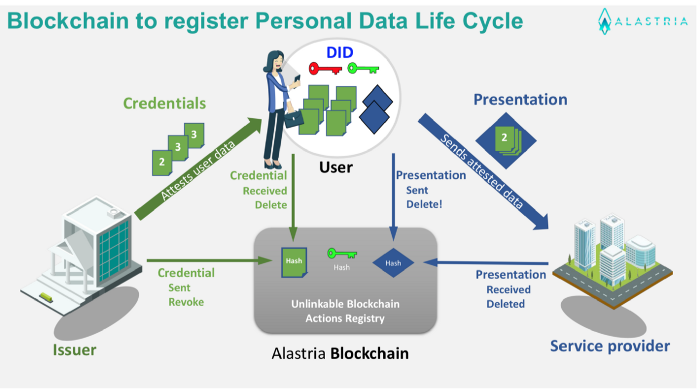
\includegraphics[width=0.8\textwidth]{rent-car-data-lifecycle.png}
            \caption{Alastria ID data life cycle}
            \label{fig:rent-cycle}
        \end{figure}
        
        Registration in the blockchain facilitates the process of checking the validity of the Credentials without the need for direct contact between the rental Service Provider and the Issuers, improving the comfort and privacy of the user (Subject), while reducing the cost and increasing the guarantees for the company.\\

        In addition, registration in the blockchain facilitates the revocation of Credentials by Issuers and the withdrawal (request for deletion) of personal data from users (Subjects).
